%%%%%%%%%%%%%%%%%%%%%%%%%%%%%%%%%%%%%%%%%%%%%%%%%%%%%%%%%%%%%%%%%%%%%%%%%%%%%%%
%% 2020-06-20
%% Descr:       Hauptdatei für die Projektarbeit / Bachelorarbeit
%% Author:      Vorlage erstellt von Daniel Spitzer an der DHBW Lörrach 
%% Angepasst: Katja Wengler, ZWI, DHBW Karlsruhe
%%%%%%%%%%%%%%%%%%%%%%%%%%%%%%%%%%%%%%%%%%%%%%%%%%%%%%%%%%%%%%%%%%%%%%%%%%%%%%%

\newif\ifseminararbeit
\newif\ifblockingnotice
%%%%%%%%%%%%%%%%%%%%%%%%%%%%%%%%%%%%%%%%%%%%%%%%%%%%%%%%%%%%%%%%%%%%%%%%%%%%%%%
%% 2020-06-20
%% Descr:       Variablen für die Projektarbeit / Bachelorarbeit festlegen
%% Author:      Vorlage erstellt von Daniel Spitzer an der DHBW Lörrach 
%% Angepasst:   Katja Wengler, ZWI, DHBW Karlsruhe
%%%%%%%%%%%%%%%%%%%%%%%%%%%%%%%%%%%%%%%%%%%%%%%%%%%%%%%%%%%%%%%%%%%%%%%%%%%%%%%

% Hier müssen die Variablen zur eignenen Arbeit angepasst werden

% Der Titel der Arbeit, der auf dem Deckblatt angezeigt wird
\def \thesisTitle {Der Titel einer wissenschaftlichen Arbeit kann auch sehr lang werden, aber länger ist nicht unbedingt besser}

% Der Titel der Arbeit, der in der Fußzeile angezeigt wird
\def \thesisFooterTitle {Der Titel einer wissenschaftlichen Arbeit kann auch sehr lang werden, aber länger ist nicht unbedingt besser}

% Art der Arbeit
\def \thesisType {1. Projektarbeit}

% Bildungsabschluss
\def \degree {Bachelor of Science (B. Sc.)}

% Abgabedatum
\def \submissionDate {31. August 2020}

% Studiengang
\def \courseOfStudies {Wirtschaftsinformatik}

% Kurs
\def \course {WWI22B5}

% Name des Autors der Arbeit
\def \name {Jona Rumberg}

% Name der Ausbildungsfirma
\def \company {SAP SE}

% Ort, an dem Ausbildungsfirma ansässig ist
\def \companyLocation {Walldorf}

% Betreuer der Ausbildungsfirma
\def \corporateAdvisor {Thomas Frambach}

% Wissenschaftlicher Betreuer
\def \universityAdvisor {Prof. Dr. Tina Mustermann}

% Ort und Datum für die Ehrenwörtliche Erklärung
\def \declarationHeading {Selbstständigkeitserklärung}
\def \declarationLocation {Karlsruhe}
\def \declarationDate {31. August 2020}

% Ort und Datum für die Freigabe der Arbeit
\def \releaseLocation {Karlsruhe}
\def \releaseDate {31. August 2020}

% Name der Bilddatei für das Firmenlogo. Die Datei muss im Ordner images sein.
% Erlaubt sind u.a. folgende Formate: PDF, PNG, JPEG
\def \fileNameLogo {SAP_R_grad_scrn.png}

% Je nach Länge des Titels kann die Schriftgröße angepasst werden
\def \titleFontSize {18}		% Schriftgröße des Titels auf dem Deckblatt
\def \footerFontSize {10}		% Schriftgröße in der Fußzeile

% Wenn es sich um eine Seminararbeit handelt,
% muss der folgende Befehl durch diesen ersetzt werden:
% \seminararbeittrue
\seminararbeitfalse

% Wenn die Arbeit keinen Sperrvermerk hat,
% muss der folgende Befehl durch diesen ersetzt werden:
% \blockingnoticefalse
\blockingnoticetrue

% Die Daten für den Sperrvermerk. Diese müssen natürlich nur geändert werden,
% wenn die Arbeit einen Sperrvermerk hat.
% Datum der Unterschrift des Autors auf dem Sperrvermerk
\def \blockingNoticeAuthorDate {31. August 2020}
% Datum der Unterschrift des Unternehmensvertreters auf dem Sperrvermerk
%\def \blockingNoticeCompanyDate {31. August 2020}

% Adresse und Land des Unternehmens auf dem Sperrvermerk. Die \\ sorgen für einen Zeilenumbruch
\def \companyAdress {Hauptstraße 1 \\ 76133 Karlsruhe \\ Deutschland}
% Telefonnummer des Unternehmens auf dem Sperrvermerk.
\def \companyPhone {0721 1234567}
% E-Mailadresse des Unternehmens auf dem Sperrvermerk.
\def \companyEmail {info@musterfrau-ag.de}
%%%%%%%%%%%%%%%%%%%%%%%%%%%%%%%%%%%%%%%%%%%%%%%%%%%%%%%%%%%%%%%%%%%%%%%%%%%%%%%
%% 2020-06-20
%% Descr:       Formale Einstellungen für die Praxisarbeit
%% Author:      Vorlage erstellt von Daniel Spitzer an der DHBW Lörrach 
%% Angepasst:   Katja Wengler, ZWI, DHBW Karlsruhe
%%%%%%%%%%%%%%%%%%%%%%%%%%%%%%%%%%%%%%%%%%%%%%%%%%%%%%%%%%%%%%%%%%%%%%%%%%%%%%%

\documentclass[a4paper,12pt]{article}
\usepackage{fontspec}
\usepackage{polyglossia}
\usepackage{csquotes}
\setdefaultlanguage[spelling=new, babelshorthands=true]{german}

% Seitenränder
\usepackage[left=3.5cm, right=2.5cm, head=1.25cm, bottom=2cm, foot=1.25cm, includefoot]{geometry}

% Abkürzungsverzeichnis
\usepackage[printonlyused]{acronym}

% Gut formatierte Tabellen
\usepackage{tabulary}

% Positioniert Tabellen und Abbildungen
\usepackage{float}

% Fügt Abschnitte wie den Anhang oder die Kurzfassung dem Inhaltsverzeichnis hinzu
\usepackage{tocbibind}

% Ermöglicht Abbildungen in LaTeX
\usepackage{graphicx}
\graphicspath{ {images/} }

% Definiert die Farben für Tabellen im DHBW-Style
\usepackage[table]{xcolor}
\definecolor{tableHeading}{gray}{0.672}
\definecolor{tableOdd}{gray}{0.945}
\definecolor{tableEven}{gray}{0.859}
\arrayrulecolor{white}

% Schriftart Carlito. Sie ist fast identisch mit Calibri.
% Calibri ist auf Linux und MacOS nicht verfügbar. 
\usepackage{carlito}
\setmainfont{carlito}

% Fußzeile und Kopfzeile
\usepackage{fancyhdr}
\renewcommand{\headrulewidth}{0pt}
\renewcommand{\footrulewidth}{0.5pt}
\def \footer{
\begin{center}
\hfill
\fontsize{\footerFontSize}{\footerFontSize}\selectfont%\thesisFooterTitle
\hfill
\thepage
\end{center}
}

% Positioniert die Fußnoten fest am unteren Ende der Seite
\usepackage[bottom]{footmisc}

% Zeilenabstand: 1.5
\usepackage{setspace}
\setstretch{1.5}

% Literaturverzeichnis
\usepackage[natbib=true, backend=biber, style=authoryear, dashed=false]{biblatex}
\DeclareBibliographyAlias{interview}{misc}
\addbibresource{text/bibliography.bib}

% Das Paket hyperref muss als letztes Paket geladen werden. Das Paket setzt Links im PDF-Dokument.
\usepackage[hidelinks, unicode]{hyperref}
\hypersetup{pdftitle = {\thesisTitle}, pdfauthor = {\name}}

% Normale Schriftart für URLs
\renewcommand{\UrlFont}{}

% Variable für das Speichern der Seitenzahl (römisch -> arabisch -> römisch)
\newcounter{pageNumber}

% Nummerierung: 2.1, 2.2 usw.
\renewcommand{\labelenumii}{\theenumii}
\renewcommand{\theenumii}{\theenumi.\arabic{enumii}.}

% Bei Bedarf können die Überschriften geändert werden
\def \declarationHeading{Selbstständigkeitserklärung}
%\def \thesisSizeHeading{Hinweis zum Umfang der Arbeit}
%\def \releaseHeading{Freigabe der Arbeit}
\def \blockingHeading{Sperrvermerk}
\def \abstractHeading{Kurzfassung}
\def \appendixHeading{Anhang}
\def \referenceHeading{Quellenverzeichnis}
\def \acronymHeading{Abkürzungsverzeichnis}

% Befehl für ein einleitendes Zitat
\newcommand{\epigraph}[2]{
    \begin{quote}\begin{quote}
        \begin{center}
            \textit{#1}
        \end{center}
        \hfill #2
    \end{quote}\end{quote}
}


\begin{document}
\thispagestyle{empty}
%%%%%%%%%%%%%%%%%%%%%%%%%%%%%%%%%%%%%%%%%%%%%%%%%%%%%%%%%%%%%%%%%%%%%%%%%%%%%%%
%% 2020-06-20
%% Descr:       Titelseite
%% Author:      Vorlage erstellt von Daniel Spitzer an der DHBW Lörrach 
%% Angepasst:   Katja Wengler, ZWI, DHBW Karlsruhe
%%%%%%%%%%%%%%%%%%%%%%%%%%%%%%%%%%%%%%%%%%%%%%%%%%%%%%%%%%%%%%%%%%%%%%%%%%%%%%%


\vspace*{-3cm}

\begin{center}


\includegraphics[width=4cm]{DHBW_logo.pdf}

\includegraphics[width=4cm]{SAP_R_grad_scrn.png}

\vspace{4cm}
\Large Fakultät Wirtschaft\\

\vspace{2cm}
\Large Studiengang \courseOfStudies \\

\fontsize{\titleFontSize}{\titleFontSize}\selectfont \thesisTitle \\

\vspace{1cm}
\thesisType \\

\normalsize Im Rahmen der Prüfung zum \degree \\

\ifblockingnotice
\vspace{0.5cm}
\Large \textcolor{red}{Sperrvermerk}\\
\vspace{0.5cm}
\else
\vspace{2cm}
\fi 


\vspace{3cm}
\submissionDate \\
\vfill
\begin{tabular}{l l}
VerfasserIn: \hspace{1cm} & \name \\
Kurs: \hspace{1cm} & \course \\ 
Dualer Partner: \hspace{1cm} & \company, \companyLocation \\
\ifseminararbeit
\else 
Betreuer der Ausbildungsfirma: \hspace{1cm} & \corporateAdvisor \\ 
\fi
Wissenschaftlicher BetreuerIn: \hspace{1cm} & \universityAdvisor \\ 
Abgabedatum: \hspace{1cm} & \submissionDate \\
\end{tabular} 
\end{center}

\pagenumbering{Roman}
\pagestyle{fancy}
\fancyhead{}
\fancyfoot{}
\fancyfoot[R]{\footer}
\newpage

%%%%%%%%%%%%%%%%%%%%%%%%%%%%%%%%%%%%%%%%%%%%%%%%%%%%%%%%%%%%%%%%%%%%%%%%%%%%%%%
%% 2020-06-20
%% Descr:       Eidensstattliche Erklärung
%% Author:      Vorlage erstellt von Daniel Spitzer an der DHBW Lörrach 
%% Angepasst:   Katja Wengler, ZWI, DHBW Karlsruhe
%%%%%%%%%%%%%%%%%%%%%%%%%%%%%%%%%%%%%%%%%%%%%%%%%%%%%%%%%%%%%%%%%%%%%%%%%%%%%%%

\begin{center}
\section*{\declarationHeading}
\addcontentsline{toc}{section}{\declarationHeading}
\end{center}
\thispagestyle{empty}
\noindent Ich versichere hiermit, dass ich die vorliegende \thesisType mit dem Thema: 

%\begin{center}
\thesisTitle
%\end{center}

\noindent selbstständig verfasst und keine anderen als die angegebenen Quellen und Hilfsmittel benutzt habe. Ich versichere zudem, dass die eingereichte elektronische Fassung mit der gedruckten Fassung übereinstimmt.

\vspace*{1.8cm}

\begin{tabular}{l c}
\noindent Karlsruhe, \declarationDate,	& \noindent\rule{9cm}{0.5pt} \\ 
 & \name \\
\end{tabular} 


\newpage

\ifblockingnotice
%%%%%%%%%%%%%%%%%%%%%%%%%%%%%%%%%%%%%%%%%%%%%%%%%%%%%%%%%%%%%%%%%%%%%%%%%%%%%%%
%% 2020-06-20
%% Descr:       Sperrvermerk
%% Author:      Vorlage erstellt von Daniel Spitzer an der DHBW Lörrach 
%% Angepasst:   Katja Wengler, ZWI, DHBW Karlsruhe
%%%%%%%%%%%%%%%%%%%%%%%%%%%%%%%%%%%%%%%%%%%%%%%%%%%%%%%%%%%%%%%%%%%%%%%%%%%%%%%

\begin{center}
\section*{\textcolor{red}{\blockingHeading}}
\addcontentsline{toc}{section}{\blockingHeading}
\end{center}

\noindent Der Inhalt dieser Arbeit darf weder als Ganzes noch in Auszügen Personen außerhalb des Prüfungsprozesses und des Evaluationsverfahrens zugänglich gemacht werden, sofern keine anders lautende Genehmigung der Dualen Partners vorliegt.

\vspace*{2cm}


\newpage
\fi

%%\section*{\abstractHeading}
\addcontentsline{toc}{section}{\abstractHeading}
Hier beginnt die Kurzfassung ihrer wissenschaftlichen Arbeit…
%%\newpage

\tableofcontents
\newpage

\section*{\acronymHeading}
\addcontentsline{toc}{section}{\acronymHeading}
\begin{acronym}

\acro{API}{Application Programming Interface}
\acro{BPMN}{Business Process Model and Notation}
\acro{ERP}{Enterprise-Resource-Planning} 
\acro{EDA}{Event Driven Architecture}
\acro{IT}{Informationstechnologie}
\acro{REST}{Representational State Transfer}
 
\end{acronym}
\newpage

\listoffigures
\newpage

\listoftables
\newpage

\clearpage
\setcounter{pageNumber}{\value{page}}
\pagenumbering{arabic}

\rowcolors{1}{tableOdd}{tableEven}

% -----------------------------------------------------
% Hier sind die Kapitel.
% Bei Bedarf kann man Kapitel entfernen oder hinzufügen
\section{Einleitung und Grundlagen der Betrachtung}
\epigraph{"`Des Menschen größtes Verdienst bleibt wohl, wenn er die Umstände soviel als möglich bestimmt und sich so wenig als möglich von ihnen bestimmen läßt."'}{Johann Wolfgang von Goethe\footcite[S. 10]{Freund2014}}
Ein zum Thema passendes Zitat fast immer eine gute Einleitung für die Arbeit. 
\ac{BPMN} ist eine Modellierungssprache.\footcite[Vgl.][S. 1]{Freund2014} Bei der ersten Verwendung von Abkürzungen werden diese in Klammern automatisch ausgeschrieben. 
Bei der zweiten Verwendung ist das nicht so, wie man anhand von \ac{BPMN} sehen kann. "`Das ist ein direktes Zitat aus dem Internet"'.\footcite[S. 3]{OMG2018}
Bei einseitigen Quellen kann man die Seitenzahl weglassen.\footcite[Vgl.][]{schlechteQuelle}
Es gibt viele schlechte Quellen.\footcite[Vgl.][S. 1-3]{schlechteQuelle2}

\subsection{Motivation und Problemstellung}
Abbildungen und Tabellen sind natürlich auch möglich.

\begin{figure}[H]
  \centering
	
\includegraphics[width=0.4\textwidth]{DHBW_logo.pdf}
   \caption[Das Logo der DHBW]{Das Logo der DHBW\footnotemark}
\end{figure}
\footnotetext{\cite[][S.1]{DHBW}}

Als Grafikformate werden u.a. PDF, PNG und JPEG akzeptiert. Die Bilddatei muss im Order "`images"' liegen.
Mit einem Label in einer Abbildung oder Tabelle kann man darauf referenzieren, wie man an der Abbildung \ref{AbbildungLogoMusterfirma} sehen kann.
\begin{figure}[H]
  \centering
	
\includegraphics[width=0.3\textwidth]{company_logo.pdf}
   \caption[Das Logo der Musterfirma]{Das Logo der Musterfirma\protect\footnotemark}
   \label{AbbildungLogoMusterfirma}
\end{figure}
\footnotetext{Eigene Darstellung in Anlehnung an \cite[S.4]{Freund2014}}

Die Breite einer Grafik oder einer Tabelle lässt sich einfach als Faktor festlegen. 1 entspricht dabei der Textbreite und 0.5 die Hälfte der Textbreite.
Bei Tabellen wird die angegebene Breite nur bei Bedarf ausgenutzt.

\begin{table}[H]
  \centering
  \begin{tabulary}{0.7\textwidth}{|L|L|}
  \hline 
  \rowcolor{tableHeading}Eigenschaft & Wert \\ 
  \hline 
  Größe & 20 cm \\ 
  \hline 
  Gewicht & 1 kg \\
  \hline
  Haarfarbe & braun \\  
  \hline 
  \end{tabulary} 
  \caption[Eine Tabelle ohne Quellenangabe]{Eine Tabelle ohne Quellenangabe}
\end{table}


Experteninterviews.\footcite[Vgl.][S. 7]{Meuser2009} Ein Zitat aus der Wirtschaftswoche.\footcite[Vgl.][S. 32]{WIWO2018}
Firmeninternes Material kann auch zitiert werden.\footcite[Vgl.][]{Firma2018} "`Das Zitat stammt aus einem Interviewprotokoll"'.\footcite{Experte2018}

Mit zwei Backslash \\ erzwingt man einen Zeilenumbruch. Bei langen Wörtern funktioniert die Worttrennung oftmals nicht mehr.
Dann muss man selbst die Silbentrennung vornehmen: Donau\-dampf\-schiff\-fahrts\-gesell\-schafts\-kapitän. \\
Aufzählungen:
\begin{itemize}
  \item Punkt 1
  \item Punkt 2
\end{itemize}
Nummerierte Aufzählung:
\begin{enumerate}
  \item Punkt 1
  \item Punkt 2
\end{enumerate}

Fußnoten sind besonders praktisch für Verweise auf andere Abschnitte der Arbeit.\footnote{Siehe Abschnitt \ref{Abschnitt:Arbeitsumfeld}} 
Mit dem ref-Befehl lassen sich Labels referenzieren. Das funktioniert bei Abbildungen, Tabellen, Kapiteln und Abschnitten.

\subsection{Zielsetung}
\subsection{Abgrenzung}
\subsection{Vorgehensweise}
\newpage
\section{Theoretischer Hintergrund}
\subsection{Event-Driven Architecture}
\subsubsection*{Ereignisse}
Zu Beginn der Betrachtung sollte der grundlegende Begriff des Ereignisses geklärt werden. Die heute gängige Definition eines Ereignisses im Kontext von \ac*{EDA} ist, dass ein Ereignis eine 'signifikante Änderung des Zustands' ist.\footcite[Vgl.][S. 4]{EDA2006} Diese relativ breite Definition hat zur Folge, dass eine große Menge an Geschäftsvorfällen als Ereignis begriffen werden kann. Als Standardbeispiel kann hier die Stornierung eines Fluges genannt werden, aber auch ein Eingang eines Auftrages, die Einstellung eines Mitarbeiters oder so etwas Reguläres wie der Beginn eines Arbeitstages, gemessen durch eine Stechuhr, konstituieren ein Ereignis. Schulte misst diesen Ereignissen in Studien für Gartner eine übergreifende Signifikanz zu. Im Grunde sei die Welt an sich ereignisgesteuert und Ereignisse als Grundlage von Architekturüberlegungen bilden diesen Umstand am besten ab. \footcite[Vgl. ][S. 2]{schulte2003growing} Mit dieser Annahme als Grundlage der Betrachtung wird noch einmal die Relevanz der Überlegungen klar. Die Modellierung von Geschäftsvorfällen, oder besser Geschäftsereignissen, in einer ereignisgesteuerten Weise bildet tatsächliche Verhältnisse akkurater und intuitiver und somit besser ab, als herkömmliche Architekturansätze. \footcite[Vgl. ][S. 13]{EDA2010} Diese Erkenntnis wird besonders relevant, wenn man betrachtet, dass mit einer wachsenden Gesamtmenge an Ereignissen die strukturierte Abarbeitung dieser immer wichtiger wird. Durch die immer ausgeprägteren \ac{IT} Landschaften von Unternehmen, die immer filigraner in der Lage sind Geschäftsvorfälle zu erfassen, oder Entwicklungen wie das Internet of Things, wächst die Datenmenge, die verarbeitet werden kann rapide. Die Interpretation dieser Daten als Ereignisse und deren strukturierte Verarbeitung stellt eine Möglichkeit dar, diese Daten sinnvoll zu nutzen und aus dieser Entwicklung Wert zu schöpfen.\footcite[Vgl. ][S. 16]{EDA2010} 
Eine im Kontext der Unternehmenssoftware relevante Unterscheidung ist dabei die zwischen technischen und Anwendungsereignissen. Anwendungsereignisse sind Ereignisse, die fachliche Bedeutung haben, wie beispielsweise 'ein Kundenauftrag geht ein', 'eine Zahlung wurde getätigt' oder 'Ein Mitarbeiter betritt das Gebäude'. Ein technisches Ereignis hingegen ist ein Ereignis, dass ausschließlich systemintern relevant ist und zu Kommunikation und Koordination von Systemkomponenten genutzt wird. Beispiele wären 'Ein Datenbankeintrag wurde erstellt' oder 'Eine Datei wurde hochgeladen'. Es ist üblich, dass Anwendungsereignisse einen höheren semantischen Stellenwert einnehmen, also dass in der Verarbeitung eines Anwendungsereignisses viele technische Ereignisse ausgelöst werden. \footcite[Vgl. ][S. 245f]{CLOUD2021}
\subsubsection*{Ereignisorientierung als Architekturansatz}
Zuerst einmal handelt es sich bei \ac{EDA}\footnote{Da sich bis jetzt keine allgemeingültige deutsche Übersetzung der Fachterminologie durchgesetzt hat, sollen in dieser Arbeit die englischen Begrifflichkeiten verwendet werden.} um ein Konzept der Prozessmodellierung. Im Gegensatz zur gewöhnlichen Ablauf-orientierten Modellierung werden die Prozesse nicht als aufeinanderfolgende Schritte, sondern als Reaktionen auf Zustände konzeptioniert. Daraus resultiert, dass nicht mehr die prozedurale Abhandlung von Arbeitsschritten die zentrale Aufgabe in der Anwendungssystem-Entwicklung darstellt, sondern die Reaktion auf Ereignisse. Im Mittelpunkt von Architekturentscheidungen steht die Frage: 'Was passiert, wenn dieses Ereignis eintritt?' und nicht mehr: 'Welche Schritte müssen zur Erfüllung dieser Anforderung gegangen werden?'. Was daraus resultiert, ist eine Architektur, die schon mit Beginn der Konzeption wesentlich agiler und robuster ist, da von Anfang an mit der Annahme gearbeitet wird, dass prinzipiell zu jedem Zeitpunkt jedes Ereignis eintreten kann.\footcite[Vgl.][S.30]{EDA2010}
Ein Definitionsversuch für \ac{EDA} könnte also wie folgt lauten: Event-Driven Archtitecture bezeichnet einen Modellierungsansatz für ein verteiltes, asynchrones System, das verschiedene Komponenten durch eine zentrale Verarbeitung von Events verbindet.\footcite[Vgl.][S. 248]{CLOUD2021}
\subsubsection*{Technische Grundkonzepte der \ac{EDA}}
\begin{figure}[H]
  \centering
	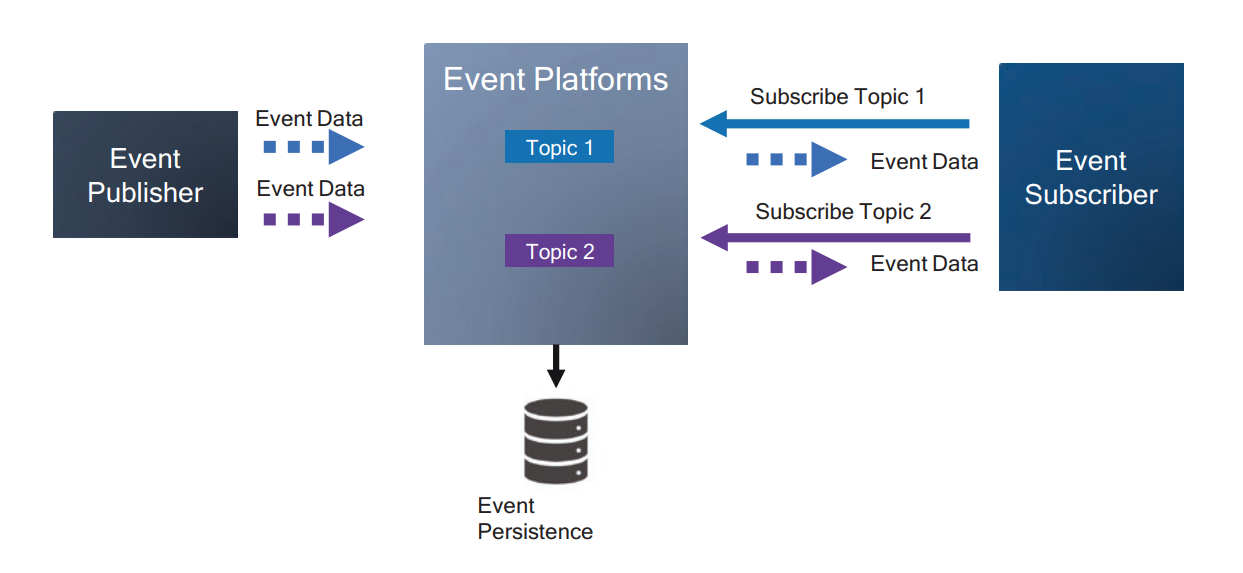
\includegraphics[width=0.8\textwidth]{Graphik EDA.png}
   \caption[Komponenten der Event-Driven Architecture]{Komponenten der \ac{EDA}\footnotemark}
\end{figure}
\footnotetext{\cite[][S. 249]{CLOUD2021}}
Die wichtigste Komponente eines durch \ac{EDA} modellierten Systems ist die zentrale Plattform zur Verarbeitung der Ereignisse in der Mitte der Architektur. Sie stellt die Infrastruktur bereit, um Events anzunehmen und diese weiterzugeben. Um einen Mehrwert aus dem System zu ziehen, muss sie darüber hinaus in der Lage sein, einen Kontext um Events herzustellen, d.h. sie in Verbindung mit anderen Ereignissen zu setzten, Ereignisse auf höheren Abstraktionsebenen zu erstellen und Ereignisse gegebenenfalls zu konsolidieren. Man spricht bei diesem Prozess von 
\ac{CEP}.\\
Weitere Komponenten des \ac{EDA} sind Publisher und Subscriber.\footnote{Für diese Komponenten finden sich in der Fachliteratur verschiedene Bezeichnungen. Außer Publisher und Subscriber findet man noch Producer und Receiver oder Producer und Listener.} Sie sind explizit von außen an das System herangeschaltet, d.h. sie haben keine Kenntnis voneinander und können auch auf völlig unterschiedlichen Plattformen basieren. Das bringt den Vorteil, dass ein durch \ac{EDA} modelliertes System inhärent modular aufgebaut ist und so zum einen weniger anfällig für Totalausfälle ist, da die Komponenten unabhängig sind, und zum anderen prädestiniert für Integrationsvorhaben ist.
Zu diesen grundlegenden Komponenten können im Zuge des \ac{CEP} noch einige weitere Konzepte hinzukommen. Die Abbildung zeigt beispielsweise eine Datenbank auf der Ereignisse persistent abgelegt werden können und die Einteilung von Ereignissen in Klassen, sogenannte Topics, die die Handhabung von verschiedenen Ereignisarten über ein System ermöglichen.\\
Hieraus ergeben sich ein paar grundlegende Fragen. Die Spezifikation der Event Platform entscheidet, wie genau Events aufgebaut sein müssen und wie Publisher und Subscriber angebunden werden. Auch weitere Überlegungen bezüglich Analyse des Ereignisflusses, Abstraktion von Ereignissen und Kompatibilität zu anderen Plattformen fallen auf Ebene der Event Platform an. Die Event Platform ist also der zentrale Baustein für die technische Umsetzung einer \ac{EDA}.\footcite[Vgl. ][S. 244]{CLOUD2021}
\subsubsection*{Technische Umsetzung von \ac{EDA}}
\label{teda}
Aus den bis hierher besprochenen Grundlagen ergeben sich einige technische Überlegungen, die bei dem Aufbau einer \ac{EDA} gefasst werden müssen.

\begin{figure}[H]
  \centering
  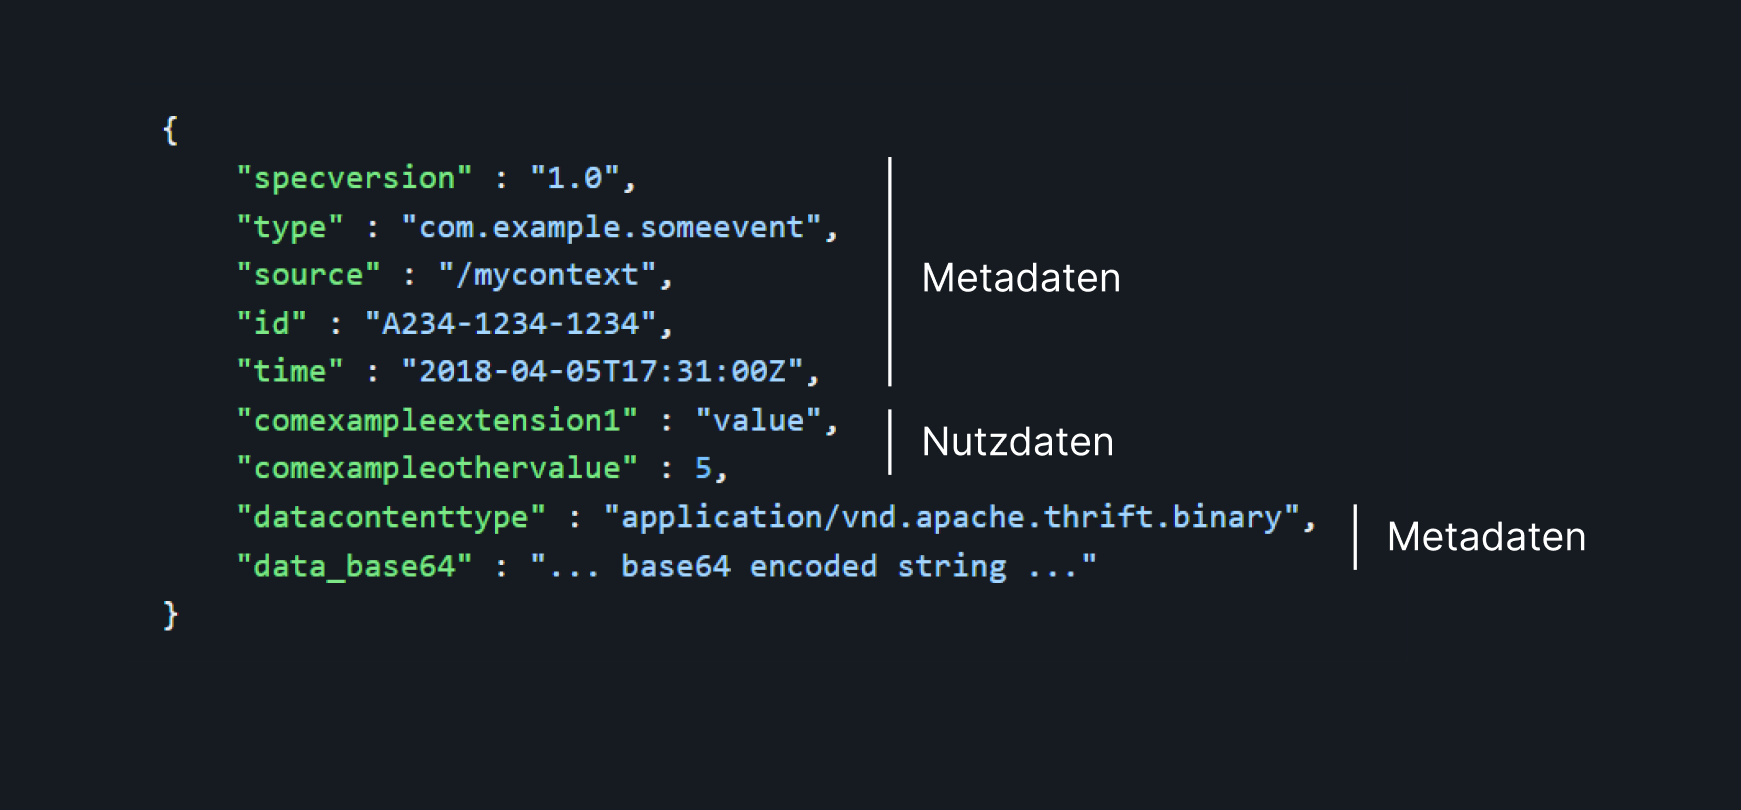
\includegraphics[width=1.0\textwidth]{Cloud Events Example.png}
  \caption[Beispiel für ein Ereignismodell]{Beispiel für ein Ereignismodell nach dem offen Standard 'CloudEvents' \footnotemark}
  \label{cloudeventslabel}
\end{figure}
\footnotetext{Eigene Darstellung nach einem Beispiel der CloudEvents Dokumentation \cite[][]{cloudeventgit}}
Ereignisse als grundlegendes Konzept der \ac{EDA} müssen in einem Ereignismodel beschrieben werden. Dieses Modell muss alle relevanten Informationen über ein Ereignis vermitteln, es sollten aber auch weitere Anforderungen an das Modell beachtet werden. Das Ereignis muss technologisch kompatibel zu allen Publishern und Subscribern sein, die an das System angeschlossen werden sollen. Es sollte zu den Nutzdaten Metadaten enthalten, die eine analytische Betrachtung des Ereignisstroms zulassen. Weiterhin sollte immer betrachtet werden, auf welcher Abstraktionsebene das Ereignis agiert, hier kann beispielsweise die technische Unterscheidung von technischen und Anwendungsereignissen sinnvoll sein. Was jedoch nie im Ereignismodell enthalten ist, ist die Verarbeitungslogik, diese liegt allein bei den Subscribern.\footcite[Vgl. ][S. 95]{EDA2010} In der Anwendung werden Ereignisse häufig als strukturierter Datentyp dargestellt, JSON oder XML als Datenformat sind üblich. Ein Beispiel findet sich in Abbildung \ref{cloudeventslabel}.

Die Architektur der Event Platform hat, wie schon angerissen, besondere Relevanz. Im Grunde unterscheiden sich zwei gängige Topologien, die hier angewandt werden können: Die 'Mediator-Topology' und die 'Broker-Topology'. 
\begin{figure}[H]
  \centering
  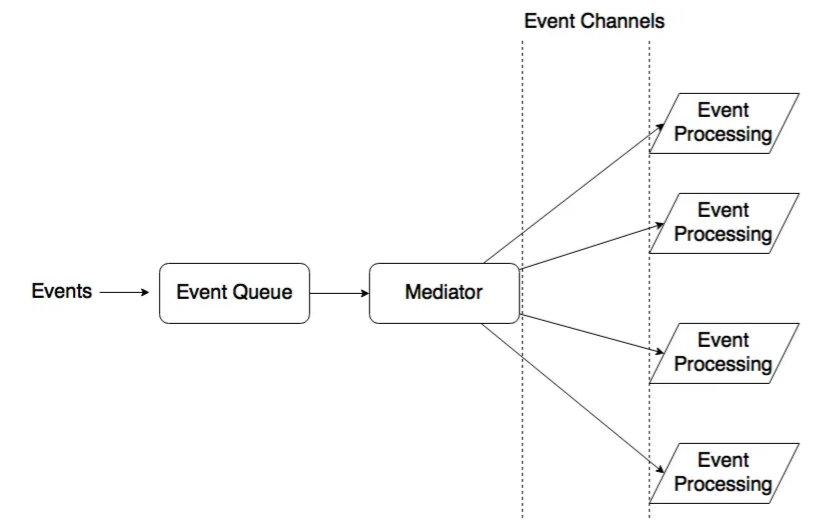
\includegraphics[width=0.8\textwidth]{Mediator Topology.png}
  \caption[Mediator-Topology]{Mediator-Topology \footnotemark}
  \label{mediatortop}
\end{figure}
\footnotetext{\cite[][]{wickramarachchi_2017_event}}
Die 'Mediator-Topology' sieht eine zentrale Event-Queue vor, in die Ereignisse eingespeist werden. Diese werden dann an die verschiedenen Subscriber verteilt, die anhand verschiedener Topics\footnote{In der Abbildung \ref{mediatortop} als Channels bezeichnet} gruppiert werden. Im Grunde werden in dieser Topologie also die ursprünglichen Ereignisse konsumiert und daraus folgend Ereignisse für jeden Channel, an den es gesendet werden soll, erzeugt und weitergegeben. Die Idee hinter diesem Prinzip ist es, auch Ereignisse, deren Verarbeitung mehrere Schritte benötigt orchestrieren zu können. \footcite[Vgl. ][]{wickramarachchi_2017_event} \\

\begin{figure}[H]
  \centering
  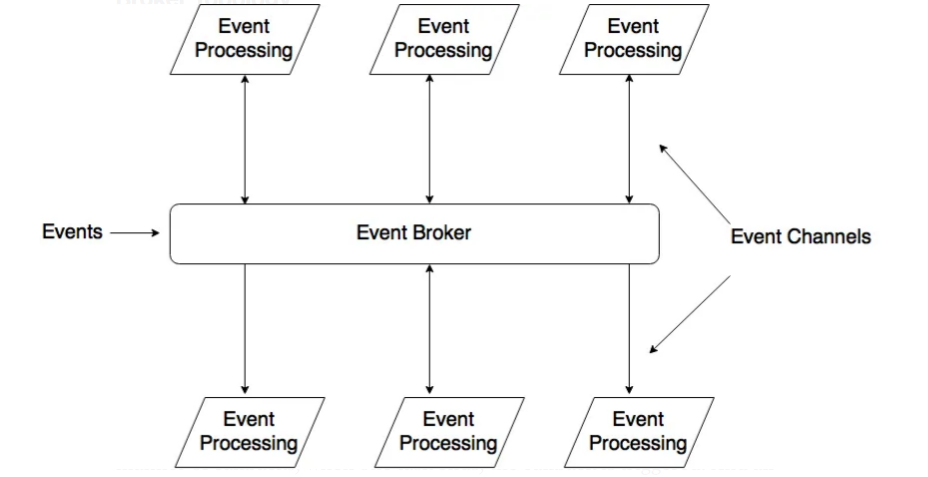
\includegraphics[width=0.8\textwidth]{Broker Topology.png}
  \caption[Broker-Topology]{Broker-Topology \footnotemark}
  \label{brokertop}
\end{figure}
\footnotetext{\cite[][]{wickramarachchi_2017_event}}
Die 'Broker-Topology' sieht keine zentrale Event-Queue vor. Hier werden die Ereignisse stattdessen zentral an alle relevanten Channels verteilt, ohne sie weiterzuverarbeiten. Daraus folgt, dass wenn Ereignisse mehrschrittig abgearbeitet werden müssen eine Lösung mit Callback-Ereignissen gefunden werden muss. In Abbildung \ref{brokertop} ist dies an Doppelpfeilen zu erkennen, die zwischen manchen Subscribern und dem Broker laufen. \footcite[Vgl. ][]{wickramarachchi_2017_event}

\subsection{RESTful API}
\subsubsection*{API}
Martin Reddy definiert in der Einleitung seines Buch "API Design for C++" den Begriff des \ac{API} als Abstraktion eines Problems und die zugehörige Spezifikation mit der ein Anwender mit einem Software-Komponenten interagieren sollte, welcher eine Lösung für dieses Problem implementiert. \footcite[Vgl. ][S. 1]{reddy2011api} Eine API ist also vordergründig eine Spezifikation, welche es ermöglicht mit Software zu interagieren. Das bedeutet sowohl, dass eine Maschine zu Maschine möglich wird, wenn die Formalisierung der Spezifikation stark genug ist, als auch, dass man nach dieser Definition eine gewöhnliche Anwendungssoftware als API, die für eine Anwender-Maschine gedacht ist, begreifen kann. Im Fachjargon der Softwareentwicklung verwendet man den Begriff der \ac{API} jedoch vordergründig, um ersteren Fall zu beschreiben. Eine praktischere Definition des Begriffes ist es also, die API als Verbindungsstück nach außen, also als Schnittstelle, einer Software-Komponente zu verstehen. \\
Eine für den Zweck der Arbeit besonders relevante Klasse von \ac{API}s sind sogenannte Web-\ac{API}s. Web-\ac{API}s sind Software-Schnittstellen, die sich das \ac{WWW} zur Nutze machen und über Protokolle des Internets angesprochen werden können.\citepls Für solche \ac{API}s haben sich über die Entwicklung des Internets eine Reihe verschiedener Standards und Architekturmuster enwtickelt, das heute eingängigste ist jedoch wahrscheinlich der REST-Standard. \citepls
\subsubsection*{REST}
Den Begriff \ac{REST} prägte erstmals Roy Fielding in seiner Dissertation im Jahr 2000. Er beschreibt damit ein Architekturprinzip für verteilte Systeme, das auf dem \ac{WWW} aufbaut. \footcite[Vgl. ][S. 76]{REST2000} \ac{API}s, die dem REST Standard folgen, sogenannte \ac{REST}ful \ac{API}s, sind mittlerweile ein häufig anzutreffendes Design Muster in der Softwarearchitektur. Dabei beschreibt Fielding mit \ac{REST} an sich eigentlich kein solches Muster, sondern legt viel mehr eine Reihe von Anforderungen fest, die erfüllt sein müssen, damit eine \ac{API} \ac{REST}ful genannt werden kann. \footcite[Vgl. ][S. XV]{richardson2007web} Die sechs Anforderungen, die Fielding definiert, sollen im folgenden kurz beschrieben werden:
\begin{itemize}
  \item 
  \textbf{Einheitliche Schnittstelle:} Die \ac{API} muss eine einheitliche Schnittstelle für alle Clients bereitstellen. Das bedeutet, dass alle Clients die gleichen Methoden verwenden, um mit der \ac{API} zu interagieren. Im Kontext des \ac{WWW} sind das beispielsweise die Methoden des \ac{HTTP} Protokolls.
  \item \textbf{Client-Server Architektur:} Die \ac{API} unterscheidet zwischen Client und Server, wobei diese Komponenten minimal gekoppelt sind, das heißt, im wesentlichen unabhängig in ihrer internen Funktionsweise. Client und Server kommunizieren über ein gemeinsames Protokoll, das ihre gesamte Abhängigkeit kapselt.
  \item \textbf{Zustandslosigkeit:} Die Kommunikation zwischen Client und Server ist zustandslos. Das bedeutet, dass der Server keine Informationen über den Zustand des Clients speichert und der Client bei jeder Anfrage alle Informationen, die der Server benötigt, um die Anfrage zu bearbeiten, mitgibt. 
  \item \textbf{Caching:} Die \ac{API} muss die Möglichkeit bieten, Antworten auf Anfragen zu cachen. Zur Optimierung des Diensts kann der Server also Daten mitgeben, die eine Gültigkeitsdauer haben und vom Client für diese Zeit zwischengespeichert werden können. Dadurch ist ein schnellerer Zugriff auf diese Daten möglich. Das Verfahren nennt man Caching.
  \item \textbf{Schichtensystem:} Die \ac{API} muss ein Schichtensystem unterstützen. Das bedeutet, dass der Client nicht direkt mit dem Server kommuniziert, sondern die Anfrage über eine Reihe von Zwischenstationen an den Server weitergeleitet werden kann. Diese Zwischenstationen können beispielsweise Firewalls oder Load Balancer sein.
  \item \textbf{Code on Demand:} Die \ac{API} muss die Möglichkeit bieten, Code an den Client zu senden, der dort ausgeführt wird. Das bedeutet, dass der Server nicht nur Daten an den Client sendet, sondern auch ausführbaren Code. Dieser Code kann dann beispielsweise die Darstellung der Daten übernehmen. Hierbei handelt es sich um die einzige optionale Anforderung, die Fielding definiert.
  \footcite[Vgl. ][]{redhat_2020_was}
\end{itemize}

\subsubsection*{RESTful APIs in der Praxis des WWW}
Seit Fielding diese Anforderung im Jahr 2000 definiert hat, ist der daraus erwachsene Design-Ansatz für APIs zu einem der populärsten Muster im Entwurf von Web-APIs geworden und die rapide Entwicklung in der IT-Branche hat natürlich auf vor diesem Thema keinen Halt gemacht. In der modernen API-Entwicklung für REST spielen sogenannte Ressourcen eine entscheide Rolle, nach denen die Struktur des Dienstes modelliert wird. Eine Ressource ist dabei ein inhaltliches Element, das Gegenstand der API ist. Eine Ressource könnte beispielsweise eine Produktinformation zu einem Produkt, der Bestand eines Lagers oder die nächste Lieferung, die im Lager eintreffen soll sein. \footcite[Vgl.][S. 81]{richardson2007web} Wird ein Dienst so modelliert, dass sich Anfragen an diesen immer auf solche Ressourcen beziehen, so lassen sich einfach die von Fielding definierten Anforderungen einhalten.

Man könnte sich als Beispiel eine Web API vorstellen, deren einzige Aufgabe es ist, die Temperaturdaten für eine spezifische Region zurückzugeben. Eine Ressource wäre also die Temperatur an einem bestimmten Ort zum aktuellen Zeitpunkt. Als Web API können inhärent die ersten beiden Punkte der Liste an Anforderungen abgehakt werden. Das Web legt eine Client-Server-Architektur zugrunde und die Kommunikation mit HTTP ist einheitlich. Interessant wird die Betrachtung der Zustandslosigkeit der API. Man könnte annehmen, dass das wechselnde Wetter durchaus einen Zustand darstellt und somit die REST Spezifikationen nicht mehr eingehalten werden. Die Definition gibt aber vor, dass Zustandslosigkeit nicht bedeutet, dass die API deterministisch sein muss, viel mehr wird nur verlangt, dass der Server keine Informationen über den Zustand des Clients speichert. Es darf also keine persistente Session geben, oder in anderen Worten, der Client muss mit jeder Anfrage sämtliche Informationen mitliefern, die der Server zur Verarbeitung derselben benötigt. Das ist hier durchaus der Fall. Der Client gibt mit jeder Anfrage an, für welchen Ort er die Temperatur zurückgegeben haben möchte. Das reicht dem Server aus, um die gefragte Information zurückzuliefern und er muss keine weiteren Informationen über den Zustand des Clients speichern. Weiterhin ist es in diesem Beispiel möglich die Temperaturdaten mit einem Gültigkeitszeitraum zu versehen, sodass Caching möglich wäre. Code on Demand wäre in diesem Beispiel nicht sinnvoll, ist aber auch nur optional.
\subsection{Technologie im Anwendungsbeispiel}

\subsubsection*{Cloud Events}
\label{cloudev}
Cloud Events sind ein Standard für ein Ereignismodell\footnote{Siehe Abschnitt \ref*{teda}}, um Ereignisse allgemeingültig beschreiben zu können. Von der Cloud Native Computing Foundation entwickelt, beschreibt er, wie Ereignisse aufgebaut sein müssen, um diese allgemeingültig verarbeiten und so eine Unabhängigkeit zwischen Publisher und Subscriber gewährleisten zu können. Der Standard hat mittlerweile weite Anwendung in der Industrie gefunden und wird unter anderen von Firmen wie Google, IBM und SAP in \ac{EDA}-Lösungen verwendet. \citepls \\
Der Standard unterstützt dabei unterschiedliche Protokolle und gibt hauptsächlich vor, welche Metadaten über das Ereignis angegeben werden müssen. So trifft er keine Aussage über die Struktur der Nutzdaten im Ereignis, sondern spezifiziert viel mehr, dass Beispielweise eine Information über den Publisher vorhanden sein muss, die Zeit und das Datum angegeben sein muss, zu der das Ereignis gesendet wurde oder eine Versionierung des Ereignisses erkennbar ist. Die Zielsetzung des Standards ist es somit nicht, inhaltliche Kompatibilität herzustellen, sondern schlicht die korrekte Verarbeitung und Weiterleitung der Ereignisse auf Seite der Event-Platform zu gewährleisten. Diese kann, da die Ereignisse, die sie verarbeitet, einem Standard folgen, Ereignisse von verschiedensten Publishern annehmen. Zudem kann, da Cloud Events für verschiedene Protokolle definiert ist, mit verschiedenen Protokollen an sie angeschlossen werden und noch mehr Unabhängigkeit geboten werden. Cloud Events selbst definiert Ziel so, "die Interoperabilität von Ereignissystemen zu definieren, die es Diensten ermöglichen, Ereignisse zu produzieren oder zu konsumieren, wobei Produzenten und Konsumenten unabhängig voneinander entwickelt und eingesetzt werden können."\citepls

\subsubsection*{RAP und Business Objects}
Das \ac{RAP} ist ein Programmiermodel, das eine Reihe von Konzepten, Sprachen und Frameworks einschließt, die zusammen die Möglichkeit bieten im SAP Umfeld Applikationen unter Verwendung der Paradigmen einer \ac*{REST}ful \ac{API} zu entwickeln. \citepls

Den Kern der Entwicklung nach diesem Modell bildet die Arbeit mit sogenannten \ac{BO}s. Es handelt sich bei diesen um das Konzept von hierarchisch aufgebauten Objekten, die den Zugriff auf Daten und Aktionen, sogenannte Behaviors zu ermöglichen. An diese \ac{BO}s lassen sich zudem weitere Dienste anknüpfen, die beispielsweise die Datenstruktur in ein User-Interface umsetzen, aus ihr eine \ac{API} generieren oder Ähnliches. Ein \ac{BO} kann dabei ein beliebiges Objekt aus der echten Welt modellieren, so könnte es beispielsweise ein Produkt, eine Reise oder einen Verkaufsabschluss mit den zugehörigen Daten repräsentieren. Unter einem Hauptknoten eines solchen Objektes hängen dann weitere zugehörige Daten, aber auch Aktionen. Bei diesen kann es sich zum Beispiel um gewöhnliche transaktionale Operationen wie erstellen, löschen oder ändern handeln, aber auch dem Anwendungsfall spezifische Operationen, wie die Weiterverarbeitung eines Produktes oder die Genehmigung einer Reise sind denkbar. Um ein \ac{BO} anzulegen, werden einige Artefakte benötigt, die wichtigsten sind dabei vielleicht die Behavior Definition und die Behavior Implementation. In ersterer wird festgelegt, welche Daten und Aktion das \ac{BO} enthält, zweitere ist eine \ac{ABAP}-Klasse, deren Methoden aufgerufen werden, wenn spezifische Aktionen des \ac{BO} von der Laufzeitumgebung angefragt werden. \citepls

\subsubsection*{Business Events}
Mit Business Events können Konzepte von \ac{EDA} im SAP Umfeld umgesetzt werden. Als Business Event wird ein Ereignis bezeichnet, das durch ein Business Object im Zuge eines Behaviors erzeugt wird. Wie in Abschnitt \ref{cloudev} bereits erwähnt, folgen solche Ereignisse im SAP Umfeld dem Standard Cloud Events. Dem Ereignis werden also einige Metadaten mitgegeben, anhand derer es weiter verarbeitet wird. Der Producer eines Business Events ist also ein Business Object. 

\subsubsection*{Event Consumption Model}
\label{ecm}
Der Subscriber im SAP Umfeld ist das sogenannte Event Consumption Model. Ähnlich wie ein Business Object handelt es sich hierbei um eine Reihe von hierarchisch miteinander verknüpften Artefakten. Bereitgestellt wird beispielsweise eine \ac{ABAP}-Klasse, die die Verarbeitung des Ereignisses übernimmt, aber auch ein Service, mit dem sich der Subscriber an die Event Platform anbinden lässt. \citepls

\subsubsection*{Event Mesh}
Die Event Platform im  SAP Umfeld setzt sich aus mehreren Teilen zusammen. Der Kern ist das sogenannte Event Mesh. Dieses ist ein Dienst der \ac{BTP}, der SAP eigenen Cloud Platform. Er ist die zentrale Instanz, die die Ereignisse annimmt und weiterleitet. Er ist in der Lage, die Ereignisse zu konsolidieren, zu filtern und zu transformieren. \citepls Weiterhin sind Event Consumption Model als Subscriber und das \ac{BO} als Publisher über verschiedene Komponenten des Enterprise Event Enablement Frameworks an den Event Mesh angebunden. \citepls

\subsection{Forschungsmethodik}
\subsubsection*{Protoyping}
\label{Protoyping}
In ihrem Buch "Wirtschaftsinformatik - Einführung und Grundlegung" definieren Heinrich u.A. einen Prototypen wie folgt: "Ein Prototyp ist ein mit geringem Aufwand hergestelltes und einfach zu änderndes, ausführbares Modell des geplanten, im Entwicklungsprozess befindlichen Systems, das erprobt und beurteilt werden kann"\footcite[S. 114]{heinrich2007wirtschaftsinformatik}
Als Methode zum Erkenntnisgewinn kann die Erstellung eines Prototypes also insofern eingesetzt werden, als das durch den explorativen Prozess des Erstellens des Prototypes sowohl über den Gegenstand des Prototypes, als auch über die Methode des Erstellens Erkenntnisse gewonnen werden können. Hierzu vor allem nicht nur die Erstellung des Prototyps selbst wichtig, sondern auch die strukturierte Bewertung des Prototyps im Nachgang.\footcite[S. 119]{heinrich2007wirtschaftsinformatik} In dieser Arbeit soll die Erstellung es solchen Prototyps dazu verwendet werden die bis jetzt theoretisch erarbeiteten Konzepte in einem praktischen Beispiel anzuwenden und so die Erkenntnisse aus der Theorie zu vertiefen.


\subsection{Zusammenfassung des theoretischen Teils}
Ereignisse im Kontext von \ac{EDA} wurden als signifikante Änderungen des Zustands definiert. Diese Ereignisse können sowohl geschäftliche Vorfälle als auch technische Ereignisse umfassen. \ac{EDA} ist ein Ansatz zur Modellierung von Prozessen, der Ereignisse statt aufeinanderfolgender Schritte in den Vordergrund stellt. In einer \ac{EDA} stellen Publisher und Subscriber die Hauptkomponenten dar, wobei die zentrale Plattform zur Verarbeitung der Ereignisse die wichtigste Komponente ist.
RESTful \ac{API}s sind eine populäre Methode für die Gestaltung von Web-\ac{API}s. Sie folgen den Prinzipien des \ac{REST}-Architekturmodells, das von Roy Fielding definiert wurde. Dieses Modell legt eine Reihe von Anforderungen fest, die eine \ac{API} erfüllen muss, um als RESTful bezeichnet zu werden.
Weiterhin wurden verschiedene Technologien und Methoden zur Umsetzung von \ac{EDA} und RESTful \ac{API}s im SAP-Umfeld vorgestellt. Dazu gehören Cloud Events, ein Standard für Ereignismodelle, das \ac{RAP} und Business Objects zur Entwicklung von Applikationen, Business Events als Konzept für \ac{EDA} im SAP Umfeld, das Event Consumption Model als Subscriber und das Event Mesh als Event Platform.
Abschließend wurde das Konzept des Prototyping als Forschungsmethode vorgestellt, das in dieser Arbeit zur Anwendung und Vertiefung der theoretischen Erkenntnisse genutzt wird. Ein Prototyp wird dabei als ein ausführbares Modell des geplanten Systems definiert, das mit geringem Aufwand erstellt und einfach geändert werden kann.
\newpage
\section{Anwendung in der Praxis}

% \subsection{Implementierung von EDA im RAP Umfeld}
\label{implementierung}
  Das Ziel dieses Abschnitts ist es, darzustellen, wie die bisher dargelegten Konzepte in der Entwicklung eines Prototyps angewandt wurden und somit ein 'Proof of Concept' erstellt wurde. Hierzu soll zuerst der Implementierungsprozess aufseiten der Event-Platform, und daran anschließend von Publisher und Subscriber dargestellt werden.

  \subsection{Implementierung aufseiten der BTP}

  Der Prototyp besteht aus einer Beispielanwendung , die auf Basis eines \ac{BO} eine Fiori UI Frontend Anwendung bereitstellt. Die Anwendung soll dabei die grundlegenden Funktionen eines \ac{BO} implementieren, also das Erstellen, Lesen, Ändern und Löschen von Datensätzen. Die Anwendung läuft auf einem SAP S/4 System und speichert Daten in der Datenbank des Systems. Zudem soll in jeder Speichersequenz des \ac{BO}s ein Business Event ausgelöst werden. An anderer Stelle im System reagiert ein Subscriber auf das Ereignis und persistiert es sowohl in einer Log-Datenbank und sendet eine Notification an einen Benutzer. \\

  Die inhaltliche Grundlage bildet nach SAP-Kovention eine Anwendung aus dem Bereich des Reisemanagements. Das \ac{BO} 'Travel' repräsentiert die Daten einer Reise. Es sollen hierbei Datensätze erstellt, verändert und gelöscht werden können. Relevant ist vor allem die Speicheraktion, denn hier soll die zusätzliche Programmlogik implementiert werden, die das Ereignis generiert. Um zu prüfen, wie mit Nutzdaten eines Ereignisses umgegangen werden muss, wird zusätzlich ein Code und eine Beschreibung in das Ereignis geschrieben.\\
  \begin{figure}
    \centering
    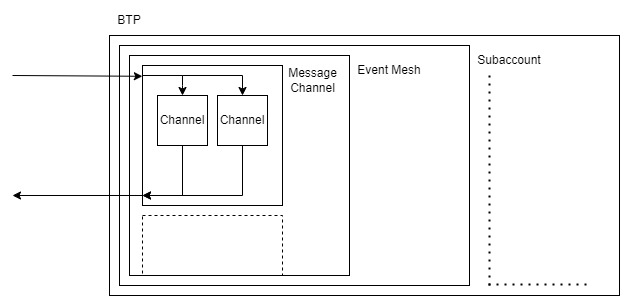
\includegraphics[width=1.0\textwidth]{event processing.jpg}
    \caption[Aufbau des BTP Event-Mesh]{Aufbau des BTP Event-Mesh \footnotemark}
    \label{EMprocessing}
  \end{figure}
  \footnotetext{Eigene Darstellung}
  Wie bereits im theoretischen Teil der Arbeit kurz angerissen und in Abbildung \ref{EMprocessing} dargestellt soll ein SAP-spezifischer Cloud-Dienst verwendet werden, der als Event-Platform fungieren soll. Die Konfiguration dieses Dienstes beginnt mit der Einrichtung eines Unteraccounts innerhalb einer \ac{BTP} Instanz. Dieser Unteraccount wird dann mit dem Event-Mesh Dienst verknüpft, der über ein User Interface administriert werden. Hier kann dann ein sogenannter Message-Client erstellt werden. Es handelt sich dabei um die aktive Komponente des Event Mesh, die Nachrichten senden und empfangen kann. Auf Ebene des Message-Clients können zudem Regeln konfiguriert werden, die Nachrichten und Ereignisse nach Themen und Absender filtern. Innerhalb des Message-Clients können dann sogenannte Queues erstellt werden. Diese Queues sind die eigentlichen Kommunikationskanäle, über die Nachrichten ausgetauscht werden. Queues horchen auf Ereignisse mit bestimmten Themen und halten diese so lange bis sie von einem Subscriber konsumiert werden.\\ 
  
  Im Folgenden soll im Kontext des Prototyps einmal durchgespielt werden, wie ein Ereignis, das durch die Änderung einer Reisebuchung ausgelöst wurde, von dem Event Mesh verarbeitet wird. Um ein Ereignis an ein Message-Channel zu senden, muss ein sogenanntes Service Binding generiert werden. Hierbei handelt es sich um ein Artefakt, 
  das in einem strukturierten Dateiformat sämtliche Verbindungs- und Authentifizierungsdaten enthält. Der Publisher kann die Informationen aus diesem Dokument, die pro Message-Channel eindeutig sind, nutzen, um eine Verbindung zum Event Mesh herzustellen. Der Publisher kann dann eine Nachricht an das Event Mesh senden. Diese Nachricht enthält neben dem eigentlichen Ereignis auch Metadaten, die das Ereignis beschreiben.  
  Hierzu gehören unter anderem das Thema des Ereignisses, der Absender und der Zeitpunkt der Erstellung. Im Kontext des Beispiels könnte das Thema des Ereignisses 'travel.booking.changed' sein, wobei das Thema aber frei wählbar ist. Um das Ereignis zu verarbeiten, müsste nun im Message Channel eine Queue konfiguriert sein, die auf dieses Thema horcht. Damit würde das Ereignis in der Queue landen und könnte von einem Subscriber konsumiert werden. 
  \begin{wrapfigure}{l}{7cm}
  \centering
  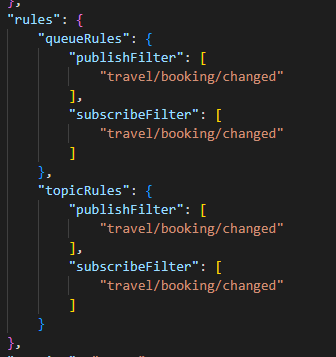
\includegraphics[width=0.4\textwidth]{messagechannelconfig.png}
  \caption[Regeln für die Konfiguration des Message-Channels]{Regeln für die Konfiguration des Message-Channels \footnotemark}
  \label{MesChannelConfig}
\end{wrapfigure}
\footnotetext{Eigene Darstellung} 
  Aufseiten des Message-Channels müsste zudem eine Regel formuliert sein, die zulässt, dass Ereignisse mit dem Thema 'travel.booking.changed' angenommen werden. Die Formulierung dieser Regeln wird bei der Erstellung des Channels im Rahmen einer Konfigurationsdatei, die service descriptor genannt wird, vorgenommen. Der service descriptor ist in Abbildung \ref{MesChannelConfig} dargestellt und erlaubt auch die Verwendung von Wildcards. Eine Regel, die im Beispiel eine Annahme des Ereignisses erlauben würde, könnte 'travel/booking/*' oder 'travel/*' sein. Im Rahmen des Prototyps wurde hierbei über die beispielhaft beschriebenen Schritte hinaus keine weitere funktionale Konfigurationsarbeit vorgenommen. Der finale Prototyp enthält eine Queue, die Ereignisse mit dem Thema 'travel.booking.changed' annimmt und eine weitere Queue, die im Grunde genau dasselbe tut, aber ausschließlich zu Testzwecken im Implementierungsprozess verwendet wurde und an die keine Subscriber angebunden wurden.\\

  Damit ist das grundlegende Gerüst der Event-Plattform fertiggestellt. An das Event Mesh können Publisher und Subscriber auf verschiedene Weisen angebunden werden. Vorgeschrieben ist nur, dass die Ereignisse, die diese erzeugen und konsumieren dem in Abschnitt \ref{cloudev} beschriebenen Cloud Event Spezifikationen folgen und somit alle relevanten Metadaten enthalten. Im Folgenden soll zuerst die Implementierung des Publishers beschrieben werden.

  \subsection{Implementierung aufseiten des SAP S/4 Systems}
  \begin{figure}
    \centering
    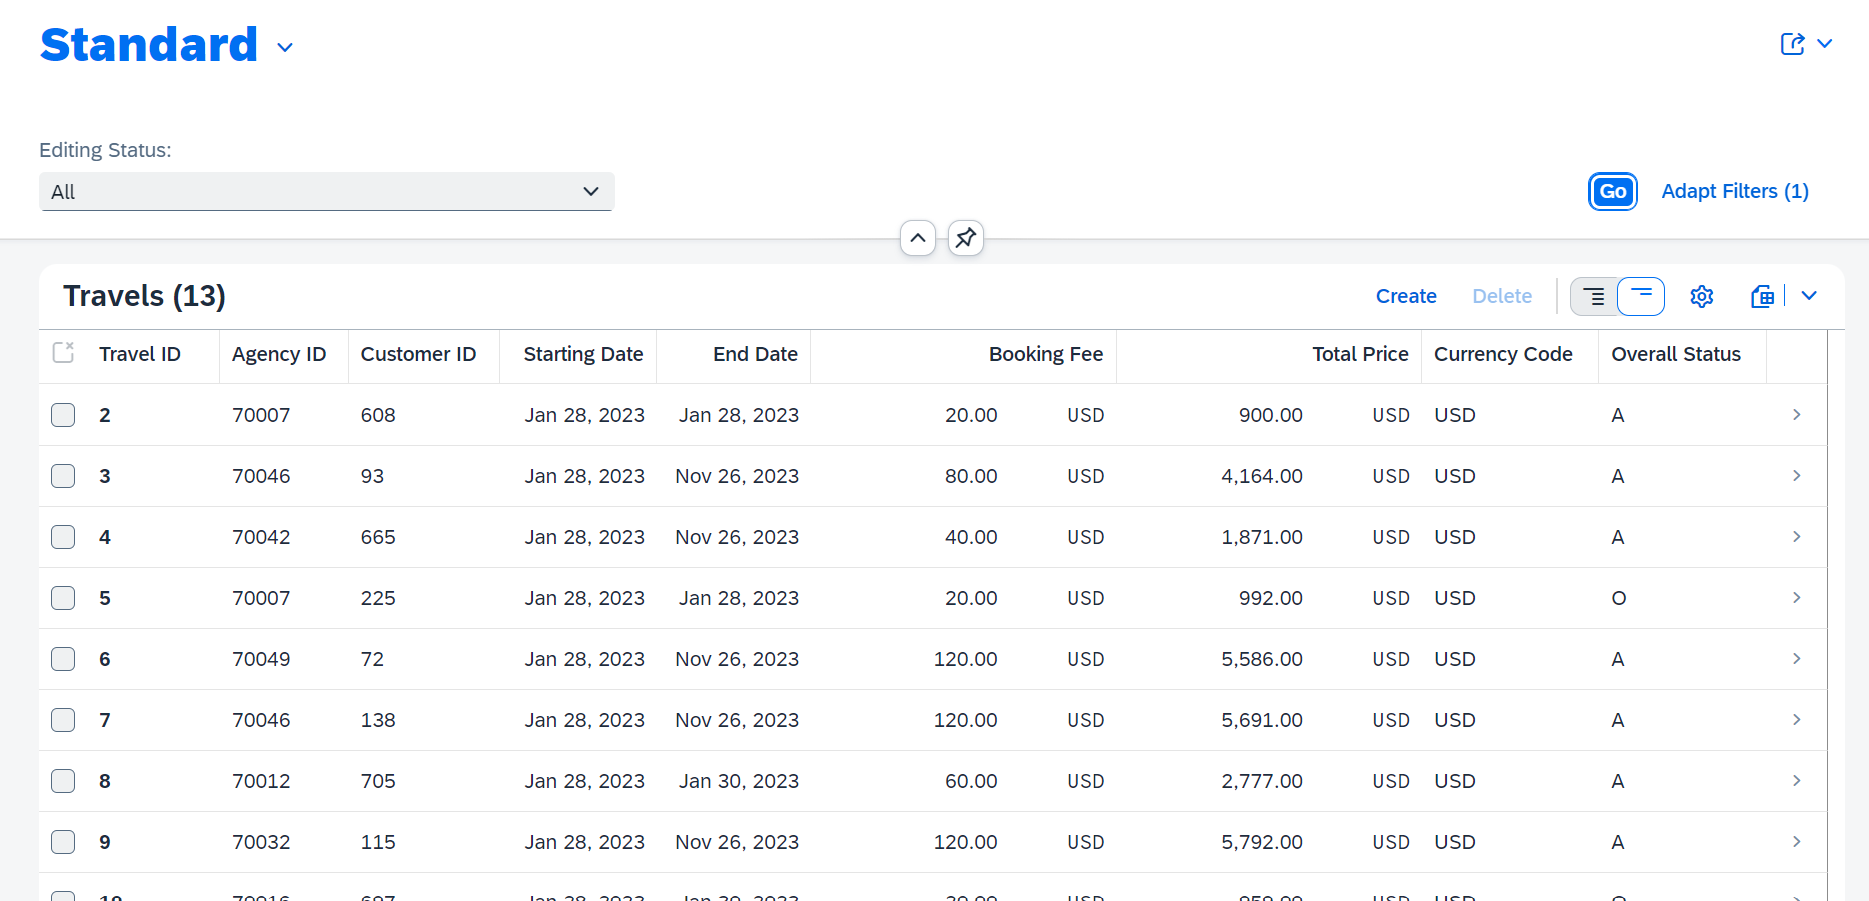
\includegraphics[width=1.0\textwidth]{fiori.png}
    \caption[Fiori Standard User Interface des Prototyps]{Fiori Standard User Interface des Prototyps \footnotemark}
    \label{fiori}
  \end{figure}
  \footnotetext{Eigene Darstellung}
  Eine simple Fiori Anwendung ist mithilfe der \ac{ADT} schnell erstellt. Auf Basis einer Tabelle als Datenquelle können alle Artefakte eines fertigen \ac{BO} generiert werden. Daraus ergibt sich eine vollständige transaktionale Anwendung, mit der Datensätze erstellt, gelesen, geändert und gelöscht werden können. Der Prototyp verwendet als Datenquelle eine Demo-Tabelle, die Reisedaten enthält. In Abbildung \ref{fiori} ist ein Auszug aus dem standardmäßig generierten User Interface dargestellt. An späterer Stelle wird noch einmal näher auf die Verwendung des \ac{BO} als Publisher eingegangen.\\

  \begin{figure}
    \centering
    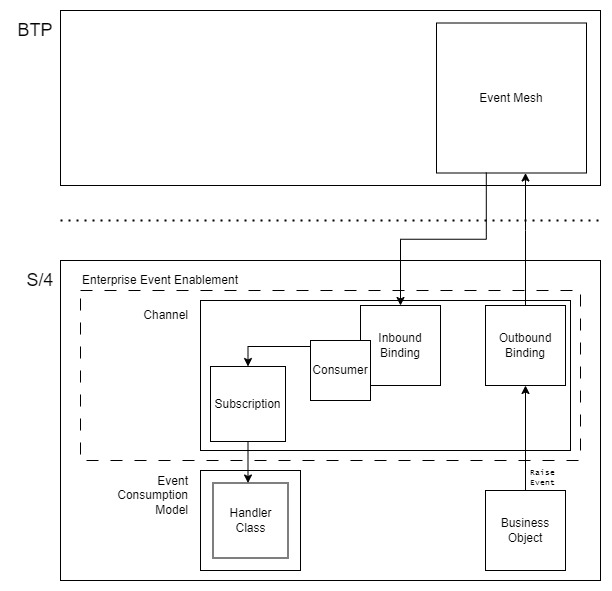
\includegraphics[width=0.7\textwidth]{eventingstructure.jpg}
    \caption[Eventing in SAP S/4 unter Verwendung des BTP Event Mesh]{Eventing in SAP S/4 unter Verwendung des BTP Event Mesh \footnotemark}
    \label{BEstructure}
  \end{figure}
  \footnotetext{Eigene Darstellung}
  Die Artefakte, die benötigt werden, um Ereignisse im S/4 System zu senden und zu empfangen sind in Abbildung \ref{BEstructure} dargestellt. Gekapselt werden sie in einem Paket, das Enterprise Event Enablement genannt wird. Für die Kommunikation mit dem Event Mesh in der Cloud muss als grundlegendes Artefakt ein Channel angelegt werden. Dieser kann automatisch generiert werden, indem der Service Key angegeben wird. Wie im vorherigen Abschnitt beschrieben, enthält dieser Service Key alle notwendigen Angaben über Endpunkte, Authentifizierung und Protokolle um sich mit dem Cloud-Service zu verbinden. Somit kann mit dem Channel diese Verbindung abgedeckt werden. Innerhalb des Channels können dann sogenannte Bindings angelegt werden. Ein Binding enthält die Konfiguration der Themen, die durch den Channel an das Event-Mesh weitergeben werden sollen.\\ Unterschieden wird in Outbound- und Inbound-Binding. Tritt im System ein Ereignis auf, das mit einem Thema im Outbound Binding übereinstimmt, kümmert sich der Channel darum, dieses an das Event Mesh weiterzugeben. Auf der anderen Seite ist das Inbound-Binding an sich auch nur eine Spezifikation von Themen, die der Channel vom Event Mesh empfangen kann. Die eigentliche Abholung der Ereignisse wird mithilfe einer Subscription konfiguriert, die die Basis für das Erstellen eines hintergründig laufenden Jobs bildet, welcher dann die Ereignisse aus der Queue des Message-Clients abholt und an die richtigen Stellen im S/4 System weiterleitet. Im Prototyp wurden also Inbound und Outbound Binding mit dem Thema 'travel.booking.changed' angelegt und zudem eine Subscription mit dem entsprechenden Thema konfiguriert.\\

Schlussendlich muss nur noch die Logik implementiert werden, die die Ereignisse auslöst und empfängt. Soll ein Ereignis durch ein \ac{BO} erzeugt werden, muss zuerst einmal in der Behavior Definition dieses \acp{BO} definiert werden, dass es ein Ereignis senden kann.\\

\begin{lstlisting}
  // dieses BO kann ein Ereignis mit dem Namen TravelCancelled senden, welches Nutzdaten vom Typ ZRU_CanceledReason enthaelt
  event TravelCancelled parameter ZRU_CanceledReason;
\end{lstlisting}

Wenn das getan ist, kann ein Artefakt, das Event-Binding, erstellt werden, welches im \ac{BO} liegt und dazu dient, Ereignisse, die im \ac{BO} erzeugt werden, an den Event-Channel weiterzugeben.\\

Im letzten Schritt muss nur noch im Programmcode der Behavior-Implementation das Ereignis auch tatsächlich ausgelöst werden. Hierzu wird das Schlüsselwort RAISE ENTITY EVENT verwendet, das als Parameter den Namen des Ereignisses und optional die Nutzdaten des Ereignisses mit dem Zusatz FROM VALUE erwartet.\\

\begin{lstlisting}[language=ABAP]
  " löst ein Ereignis mit einem Parameter aus
  RAISE ENTITY EVENT zru_r_traveltp~TravelCancelled
  FROM VALUE #( ( TravelID = 4 %param ='aTestEvent' ) ).
\end{lstlisting}

Wird dieser Programmcode ausgeführt, wird das Ereignis ausgelöst und mithilfe der bis jetzt besprochenen Artefakte an das Event Mesh weitergegeben.\\

Es bleibt zu beleuchten, wie ein Ereignis in S/4 konsumiert wird. Wenn Inbound-Binding sowie Subscription definiert sind, kann mithilfe der \ac{ADT} ein Event Consumption Model angelegt werden. Wie bereits in Abschnitt \ref{ecm} dargestellt handelt es sich hierbei um eine Sammlung von Artefakten, deren relevanteste Aufgabe es ist, eine \ac{ABAP}-Klasse bereitzustellen, deren Methoden immer dann aufgerufen werden, wenn ein Ereignis konsumiert wurde. Zur Generation dieses Event Consumption Models wird eine strukturierte Beschreibung des Ereinisses benötigt, welches verarbeitet werden soll. Im SAP Kontext erfolt diese Beschreibung nach dem offenen Standart von AsyncAPI.\footnote{Auf diesen Standard soll an dieser Stelle nicht näher eingegangen werden, da das Artefakt, das ein Ereignis beschreibt in den allermeisten Fällen automatisch generiert werden kann.} Mithilfe dieser Ereignisbeschreibung kann dann ein Event Consumption Model generiert werden. Teil dieses Models ist eine Klasse, in der schlussendlich eine Methode implementiert werden kann, die immer dann aufgerufen wird, wenn ein Ereignis konsumiert wurde. Der Quellcode aller Artefakte des Prototyps ist im Anhang zu finden.\\

Mit diesem Prototyp wurde vor allem gezeigt, wie es möglich ist, im gegeben Softwareumfeld eine \ac{EDA} zu implementieren. Zudem wurde eine Übersicht über die Schritte gewonnen, die nötig sind um Das zu erreichen. Bezogen auf das einleitend erwähnte Problem wurde gezeigt, dass es möglich ist asynchron, aus der Speichersequenz eines \ac{BO} heraus, die Speichersequenz eines anderen Komponenten aufzurufen. Explizit wurde hier implementiert, dass, wenn ein BO vom Typ travel neu angelegt wird ein Ereignis ausgelöst wurde. Das Coding hierfür stellt die einzige zusätzliche Logik im BO da, was dazu führt, dass nach seiner Ausführung der Speicherprozess eingeleitet wird. Die Verarbeitung des Ereignisses erfolgt im weiteren Verlauf asynchron.
Davon abstrahierend kann bezüglich der Forschungsfrage eingeordnet werden, dass das betrachtete System durchaus ein komplexes System darstellt, was im folgenden Kapitel eine Bewertung in diesem Kontext und eine weitere Bearbeitung der Forschungsfrage zulässt.\\
\newpage
\section{Diskussion der Ergebnisse}
\subsection{Beurteilung von EdA. und REST}
\subsection{Bewertung des Prototyps} 
\subsection{Chancen der Technologie im betriebswirtschaftlichen Kontext}

\newpage
\section{Fazit}

 





% -----------------------------------------------------

\label{pagesForDeclaration}

\clearpage
\pagenumbering{Roman}
\setcounter{page}{\value{pageNumber}}

\section*{\referenceHeading}
\addcontentsline{toc}{section}{\referenceHeading}
\defbibheading{books}{\noindent\large\textbf{Bücher}}
\printbibliography[type=book, heading=books]

\defbibheading{incollection}{\noindent\large\textbf{Sammelwerke}}
\printbibliography[type=incollection, heading=incollection]

\defbibheading{article}{\noindent\large\textbf{Artikel}}
\printbibliography[type=article, heading=article]

\defbibheading{conference}{\noindent\large\textbf{Konferenzen}}
\printbibliography[type=conference, heading=conference]

\defbibheading{online}{\noindent\large\textbf{Internetquellen}}
\printbibliography[type=online, heading=online]

\defbibheading{interview}{\noindent\large\textbf{Interviews}}
\printbibliography[type=interview, heading=interview]

\defbibheading{internal}{\noindent\large\textbf{Interne Quellen}}
\printbibliography[type=unpublished, heading=internal]
\newpage

\section{\appendixHeading}
% \addcontentsline{toc}{section}{\appendixHeading}


 
\end{document}